\documentclass{article}

\date{}
\pagestyle{empty}
\usepackage{tikz}
\title{MAS341 Graph Theory: Homework 2}


\begin{document}
\maketitle
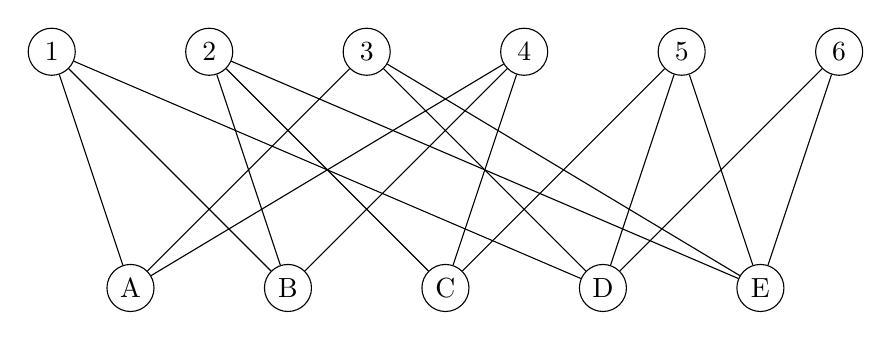
\begin{tikzpicture}[rotate=90]
\tikzstyle{vertex}=[circle, draw, minimum size=17pt, inner sep=0pt]
\node[vertex] (A) at (0,9) {A};
\node[vertex] (B) at (0,7) {B};
\node[vertex] (C) at (0,5) {C};
\node[vertex] (D) at (0,3) {D};
\node[vertex] (E) at (0,1) {E};

\node[vertex] (1) at (3,10) {1};
\node[vertex] (2) at (3,8) {2};
\node[vertex] (3) at (3,6) {3};
\node[vertex] (4) at (3,4) {4};
\node[vertex] (5) at (3,2) {5};
\node[vertex] (6) at (3,0) {6};

\draw (A)--(1)--(B)--(2)--(C)--(5)--(E)--(6)--(D)--(3)--(A)--(4)--(B);
\draw (C)--(4);
\draw (3)--(E)--(2);
\draw (1)--(D)--(5);

\end{tikzpicture}

All questions use the graph $\Gamma$ shown above.

\begin{enumerate}
\item Show that $\Gamma$ isn't Hamiltonian, using the fact that it's bipartite
\item Find a clsoed walk that uses every vertex but vertex 4 exactly once, and by adapting the Planarity Algorithm for Hamiltonian graphs, prove that $\Gamma$ isn't planar (the argument begins: if it were drawn on the plane, the closed walk you found would be a circle.  Now, vertex 4 must be inside or outside the circle... )
\item Give another proof that $\Gamma$ isn't planar using Kuratowski's theorem
\item Let $e$ be the edge connecting vertices D and 5.  Show that if we remove $e$, the resulting graph $\Gamma\setminus e$ is planar by drawing it on the plane, being sure to label your vertices.
\end{enumerate}
  


\end{document}
